\documentclass[tikz,border=8pt]{standalone}
% Shared look for every TikZ diagram. Load with \input{../../tools/tikz-style.tex}
\usepackage[sfdefault]{roboto}
\usetikzlibrary{arrows.meta, positioning, shapes.geometric, calc, fit, backgrounds}
\definecolor{cblue}{HTML}{4C78A8}
\definecolor{corange}{HTML}{F58518}
\definecolor{cgreen}{HTML}{54A24B}
\definecolor{cred}{HTML}{E45756}
\definecolor{cpurple}{HTML}{B279A2}
\definecolor{cgrey}{HTML}{6B6B6B}
\tikzset{
  every picture/.style={font=\sffamily, line width=1.2pt},
  box/.style={draw=#1, fill=#1!12, rounded corners=4pt, align=center, inner sep=7pt, minimum height=1.1cm},
  box/.default=cgrey,
  arrow/.style={-{Stealth[length=3mm]}, draw=cgrey, line width=1.4pt},
  title/.style={font=\sffamily\bfseries\Large},
  note/.style={font=\sffamily\small, text=cgrey, align=center},
}
\AtBeginDocument{\hyphenpenalty=10000 \exhyphenpenalty=10000}

% What goes into Nav2's controller server with DWB, and what comes out (navigation2 main, 2026-10-12):
% controller_frequency 20 Hz (parameter_handler.cpp); local costmap: rolling 3 m x 3 m, 0.05 m cells, updated at
% 5 Hz (nav2_bringup nav2_params.yaml); the global plan comes with the FollowPath action from the behaviour tree,
% which remakes it once a second (navigate_to_pose_w_replanning_and_recovery.xml, RateController hz 1.0);
% odometry gives the measured speed; out: cmd_vel, one (v, omega) per cycle.
\begin{document}
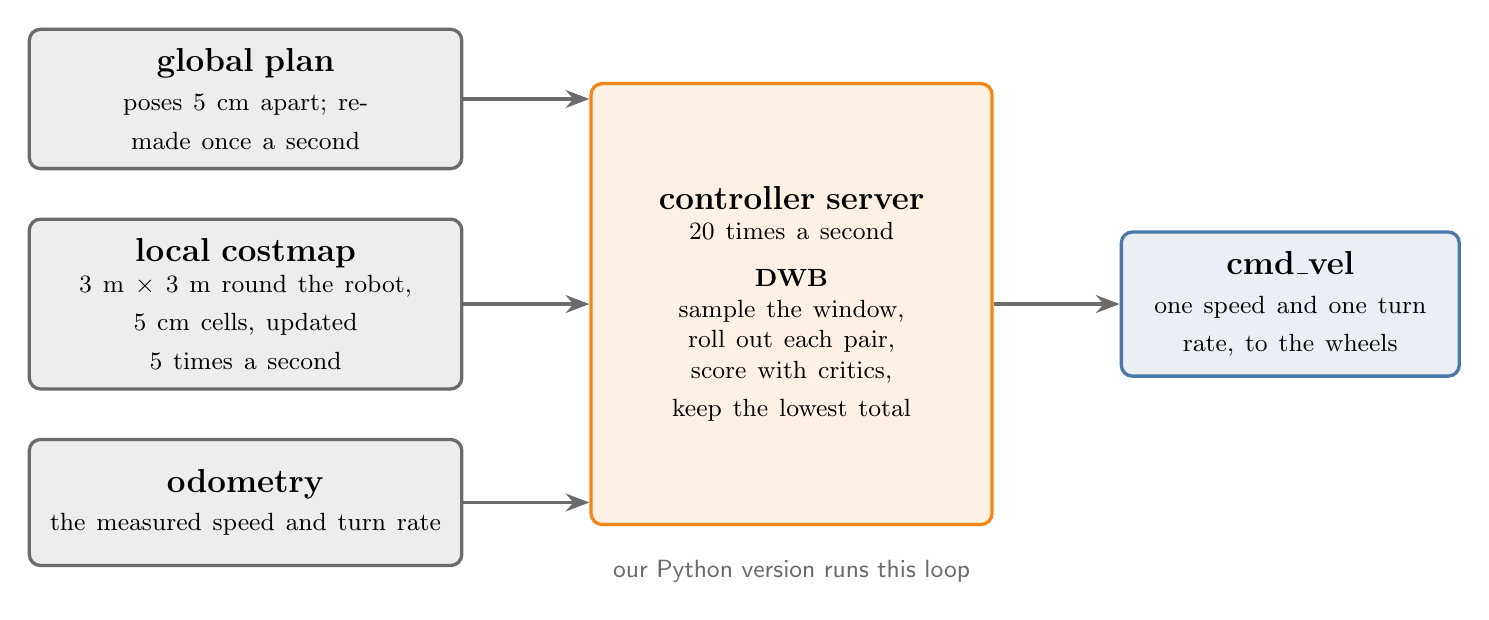
\begin{tikzpicture}[every node/.append style={font=\large}, node distance=0.6cm,
  st/.style={box=#1, minimum width=5.4cm, text width=5.0cm, minimum height=1.6cm}]
  \node[st=cgrey] (plan) {\textbf{global plan}\\ \small poses 5 cm apart; remade once a second};
  \node[st=cgrey, below=of plan] (cost) {\textbf{local costmap}\\ \small 3 m $\times$ 3 m round the robot,\\ 5 cm cells, updated 5 times a second};
  \node[st=cgrey, below=of cost] (odom) {\textbf{odometry}\\ \small the measured speed and turn rate};
  \node[st=corange, right=1.6cm of cost, minimum height=5.6cm, text width=4.6cm, minimum width=5.0cm] (dwb)
    {\textbf{controller server}\\ \small 20 times a second\\[6pt] \textbf{DWB}\\ \small sample the window,\\ roll out each pair,\\ score with critics,\\ keep the lowest total};
  \node[st=cblue, right=1.6cm of dwb, minimum width=4.2cm, text width=3.8cm] (cmd) {\textbf{cmd\_vel}\\ \small one speed and one turn rate, to the wheels};
  \draw[arrow] (plan.east) -- (dwb.west |- plan.east);
  \draw[arrow] (cost) -- (dwb);
  \draw[arrow] (odom.east) -- (dwb.west |- odom.east);
  \draw[arrow] (dwb) -- (cmd);
  \node[note, below=0.3cm of dwb, text width=5.6cm] {our Python version runs this loop};
\end{tikzpicture}
\end{document}
